\documentclass[a4paper, 12pt]{report}
\usepackage[utf8]{inputenc}
\usepackage[french]{babel}
\usepackage[pdftex]{graphicx}
\usepackage{fancyhdr}
\usepackage{algorithm}
\usepackage{algorithmic}
\usepackage{cite}
\usepackage{microtype}
\usepackage{makecell}
\usepackage{hyperref}


%\pagestyle{fancy}

\newcommand{\esp}{\textsc{esp32}}
\newcommand{\espmesh}{\textsc{esp-mesh}}
\newcommand{\mac}{\textsc{mac}}
\newcommand{\rssi}{\textsc{rssi}}
\begin{document}
%\pagenumbering{roman}

\begin{titlepage}
\begin{center}

{\Large Université de Mons}\\[1ex]
{\Large Faculté des sciences}\\[1ex]
{\Large Département d'Informatique}\\[1ex]
{\Large Service de réseaux et télécommunications}\\[2.5cm]

\newcommand{\HRule}{\rule{\linewidth}{0.3mm}}
% Title
\HRule \\[0.3cm]
{ \LARGE \bfseries Réseau Wi-Fi multi-sauts sur plateforme ESP \\[0.3cm]}
{ \LARGE \bfseries Rapport de projet \\[0.1cm]}
\HRule \\[1.5cm]

% Author and supervisor
\begin{minipage}[t]{0.45\textwidth}
\begin{flushleft} \large
\emph{Directeur:}\\
Bruno \textsc{Quoitin}
\end{flushleft}
\end{minipage}
\begin{minipage}[t]{0.45\textwidth}
\begin{flushright} \large
\emph{Auteur:} \\
Arnaud \textsc{Palgen}
\end{flushright}
\end{minipage}\\[2ex]

\vfill

% Bottom of the page
\begin{center}
\begin{tabular}[t]{c c c}

\includegraphics[height=1.5cm]{images/logoumons.jpg} &
\hspace{0.3cm} &

\includegraphics[height=1.5cm]{images/logofs.jpg}
\end{tabular}
\end{center}~\\
 
{\large Année académique 2019-2020}

\end{center}
\end{titlepage}
\tableofcontents
\chapter{Etat de l'Art}

\section{ESP-MESH}
    \espmesh\ est le protocol du constructeur Espressif permettant d'établir un réseau mesh avec des \esp.
    Cette section explique le fonctionnement de ce protocole.\\
    La topologie ici utilisée est l'arbre. La racine de l'arbre est la seule interface entre le
    réseau \espmesh\ et le reste du réseau.\\

    \textbf{Construction d'un réseau}
    \newline
    \begin{enumerate}
        \item \'Election de la racine
            \begin{itemize}
                \item Sélection automatique\\
                    Chaque noeud se trouvant à l'état idle va transmettre son addresse \mac\ et la
                    la valeur de son \rssi\ avec le routeur via des beacons.\\
                    Simultanément, chaque noeud scan les beacons des autres noeuds. Si un noeud
                    en détecte un autre avec un \rssi\ plus fort, il va transmettre le contenu des
                    ce beacon (càd voter pour ce noeud).\\
                    Ce processus sera répété pendant un nombre minimum d'itérations.\\
                    Après toutes les itérations, chaque noeud va calculer le ratio
                    \[\frac{nombre\ de\ votes}{nombre\ de\ noeuds\ participants\ \textrm{\textit{à l'élection}}}\]
                    Si ce ratio est au dessus d'un certain seuil, ce noeud deviendra la racine.

                \item Sélection par l'utilisateur\\
                    La racine se connecte au routeur et elle ainsi que les autres noeuds, oublient le processus
                    délection.
            \end{itemize}
        \item Formation de la deuxième couche\\
            Les noeuds dans l'état idle à portée de la racine vont s'y connecter et devenir des noeuds intermédiaires.
        
        \item Formation des autres couches\\
            Les noeuds dans l'état idle à portée de noeuds intermédiaires vont s'y connecter. Si plusieurs parents
            sont possibles, un noeud choisira son parent selon deux critères:
            \begin{enumerate}
                \addtolength{\itemindent}{1cm}
                \item[1.] La couche sur laquelle se situe le candidat parent:
                    le candidat se trouvant sur la couche la moins profonde sera choisi. 
                \item[2.] Le nombre d'enfants du candidat parent: si plusieurs candidats se trouvent
                    sur la couche la moins profonde, celui avec le moins d'enfants sera choisi. 
            \end{enumerate}
            Une fois connecté, les noeuds deviendront des noeuds intermédiaires si le nombre maximale de couche n'est pas atteint.
            Sinon, les noeuds de la dernière couche deviendront automatiquement
            des feuilles, empêchant d'autres noeuds dans l'état idle de s'y connecter.

    \end{enumerate}
    Pour éviter les boucles, un noeud ne va pas se connecter à un noeud dont l'adresse \mac\ se trouve dans sa table de routage.
    \vspace{0.5cm}

    \textbf{Routage}\newline
        \begin{enumerate}
            \item Table de routage\\
                Chaque noeud possède sa table de routage. Soit $p$ un noeud, sa table de routage contient les addresses \mac\ 
                des noeuds du sous-arbre ayant $p$ comme racine, et également celle de $p$.\\
                Elle est partitionnée en sous-tables qui correspondent au sous-arbres des enfants de $p$.
            \item Protocole de routage\\
                Quand un paquet est reçu,
                \begin{itemize}
                    \item Si l'adresse \mac\ du paquet est dans la table de routage et si elle est différente de l'adresse du noeud l'ayant reçu, le paquet est envoyé
                    à l'enfant correspondant à la sous-table contenant l'adresse.
                    \item Si l'adresse n'est pas dans la table de routage, le paquet est envoyé au parent.
                \end{itemize}
                \espmesh\ utilise un mécanisme de vérification de chemin pour détecter les boucles. Si une boucle arrive, un parent va prévenir son enfant et initier une déconnexion.

        \end{enumerate}
        \vspace{0.5cm}
    \newpage
    \textbf{Mise sous tension asynchrone}\newline
        La structure du réseau peut être affectée par l'ordre dans lequel les noeuds sont mis sous tension.
        Les noeuds ayant une mise en tension retardée suivront les deux règles suivantes:
        \begin{enumerate}
            \item Si une racine existe déja, le noeud ne vas pas essayer d'élir une nouvelle racine
                même si son \rssi\ avec le routeur est meilleur. Il va rejoindre le réseau comme un noeud
                dans l'état idle. \\
                Si le noeud est la racine désignée, tous les autres noeuds vont rester dans l'état idle
                jusqu'a ce que le noeud soit mis en tension.
            \item Si le noeud devient un noeud intermédiraire, il peut devenir le meilleur parent d'un autre noeud ( cet autre noeud changera donc de parent).
            \item Si un noeud dans l'état idle a un parent prédéfini et que ce noeud n'est pas sous tension, il ne vas pas essayer de se connecter à un autre parent.
        \end{enumerate}
    \vspace{0.5cm}
    \textbf{Défaillance d'un noeud}\newline
        \begin{itemize}
            \item Défaillance de la racine\\
                Si la racine tombe, les noeuds de la deuxième vont d'abord tenter de s'y reconnecter.
                Après plusieurs essais ayant échoué, les noeuds de la deuxième couche vont entammer entre eux, le processus d'élection d'un nouvelle racine.\\
                Si la racine ainsi que plusieurs couches tombent, le processus d'élection sera initialisé sur la couche la plus haute.


            \item Défaillance d'un noeud intermédiaire\\
                Si un noeud intermédiaire tombe, ses enfants vont d'abord tenter de s'y reconnecter.
                Après plusieurs essais ayant échoué, ils se connecteront au meilleur parent disponible.\\
                S'il n'y a aucun parent possible, ils se mettront dans l'état idle.
        \end{itemize}
        \vspace{0.5cm}
        \textbf{Changement de racine}\newline
            Un changement de racine n'est possible que dans deux situations:
            \begin{enumerate}
                \item La racine tombe. (voir point précédent)
                \item La racine le demande.
                    Dans ce cas, un processus d'élection de racine sera initialisé. La nouvelle racine élue
                    enverra alors une switch request à la racine actuelle qui répondra par un aquitement.
                    Ensuite la nouvelle racine se déconnectera de son parent et se connectera au routeur.
                    L'ancienne racine se déconnectera du routeur et rentrera dans l'état idle pour enfin se connecter à un nouveau parent.
            \end{enumerate}
    \newpage
    \textbf{Paquets ESP-MESH}\\
        Les paquets \espmesh\ sont contenu dans une trame wifi. Une transmission mutli-sauts utilisera un paquet \espmesh\ transporté entre chaque noeuds par un paquet wifi différent.\\
        La figure \ref{fig_meshPacket} montre la structure d'un paquet \espmesh:\\

        \begin{figure}[h]
            \centering
            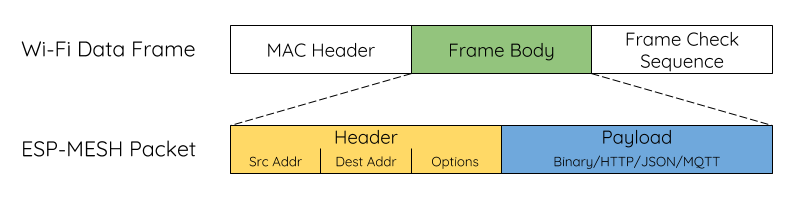
\includegraphics[scale=0.5]{images/mesh-packet.png}
            \caption{Paquet \espmesh\ \cite{ESP-MESH}}
            \label{fig_meshPacket}
        \end{figure}
        Le header d'un paquet \espmesh\ contient les adresses \mac\ source et destination ainsi que diverse options.\\
        Le payload d'un paquet \espmesh\ contient les données de l'application.
    
    \vspace{0.5cm}
    \textbf{Multicasting}\\
        Le multicasting permet d'envoyer simultanément un paquet \espmesh à plusieurs noeud du réseau. Le multicasting
        peut être réalisé en spécifiant
        \begin{itemize}
            \item Soit un ensemble d'adresses \mac\\
                Dans ce cas, l'adresse de destination doit être
                {\fontfamily{qcr}\selectfont \textls[-300]{\small 0 1 : 0 0 : 5 E : x x : x x : x x}}
                Cela signifie que le paquet est un pquet multicast et que la liste des adresses peut être obtenue dans les options du header.
            \item Soit un groupe préconfiguré de noeuds\\
                Dans ce cas, l'adresse de destination du paquet doit être l'ID\footnote{Dans un réseau\espmesh, chaque groupe a un ID unique}
                du groupe et un flag \textsc{mesh\_data\_group} doit être ajouté.
        \end{itemize}

    \vspace{0.5cm}
    \textbf{Broadcasting}\\
        Le broadcasting permet de transmettre un paquet \espmesh\ à tous les noeuds du réseau. Pour éviter de gaspiller de
        la bande passante, \espmesh utilise les règles suivantes:
        \begin{enumerate}
            \item Quand un noeud intermédiare reçoit un paquet broadcast de son parent, il va le transmettre à tous ses enfants
                et en stocker une copie
            \item Quand un noeud intermédiaire est la source d'un paquet broadcast, il va le transmettre à son parent et à ses enfants
            \item Quand un noeud intermédiaire reçoit un paquet d'un de ses enfants, il va le transmettre à ses autres enfants, son parent
                et en stocker une copie
            \item Quand une feuille est la source d'un paquet broadcast, elle va le transmettre à son parent
            \item Quand la racine est la source d'un paquet broadcast, elle va le transmettre à ses enfants
            \item Quand la racine reçoit un paquet broadcast de l'un de ses enfants, elle va le transmettre à ses autres enfants et en stocker une copie
            \item Quand un noeud reçoit un paquet broadcast avec son addresse \mac\ comme adresse source, il l'ignorer
            \item Quand un noeud intermédiaire reçoit un paquet broadcast de son parent, qui a été à l'origine transmis par l'un de ses enfants, il va l'ignorer
        \end{enumerate}
    \vspace{0.5cm}
    \textbf{Contrôle de flux}\\
        Pour éviter que les parents soient submergés de flux venant de leurs enfants, chaque parent va
        assigner une fenêtre de réception à chaque enfant. Chaque noeud enfant doit demander une une fenêtre
        de réception avant chaque transmission. La taille de la fenêtre peut être ajustée dynamiquement.
        Une transmission d'un enfant vers un parent se déroule en plusieurs étapes:
        \begin{enumerate}
            \item Le noeud enfant envoit à son parent une requête de fenêtre. Cette requête contient le numéro de séquence du paquet en attente d'envoi.
            \item Le parent reçoit la requête et compare le numéro de séquence avec celui du précédent paquet envoyé par l'enfant.
                La comparaison est utilisée pour calculer la taille de la fenêtre qui est transmise à l'enfant.
            \item L'enfant transmet le paquet en accord avec la taille de fenêtre. Une fois la fenêtre de réception utilisée, l'enfant doit renvoyer une demande de fenêtre.
        \end{enumerate}
    \vspace{0.5cm}
    \textbf{Performances}\\
        Espressif fournit les performances d'\espmesh\ pour un réseau de 100 noeuds avec un nombre maximum de couches de 6 et un nombre d'enfants maximum par noeuds de 6.
        \newline

        %\vspace{0.5cm}
        \begin{tabular}{|l|l|}
            \hline
            Temps de construction du réseau & $<$ 60 secondes\\ \hline
            Latence par saut & 10 à 30 millisecondes\\ \hline
            Temps de réparation du réseau & \makecell{Si la racine tombe: $<$ 10 secondes \\ Si un noeud enfant tombe: $<$ 5 secondes}\\ \hline
        \end{tabular}

%\listoffigures
\bibliography{biblio.bib}{}
\bibliographystyle{plain}

\end{document}